\subsubsection{Motenge-Boma-Gruppe}\label{sec:MTB-Gr}

Die Motenge-Boma-Gruppe beschreibt eine subrezente keramische Stilgruppe mit einem sehr begrenzten Verbreitungsgebiet am mittleren bis oberen \mbox{Ubangi} (Abb.~\ref{fig:MTB_Verbreitung}), die sich durch intensiven Gebrauch von Schnitzroulette sowie einen diagnostischen Korpus aus charakteristischen Gefäß- und Randformen auszeichnet (Abb.~\ref{fig:MTB_Typvertreter}). Keramik der Motenge-Boma-Gruppe wurde erstmals durch Francis~L. \textcites[75]{vanNoten.1978}[69]{vanNoten.1982d} beschrieben, der im Rahmen einer Prospektion entlang des \mbox{Ubangi} zwischen Dezember 1972 und März 1973 einen Survey sowie kleinere Testgrabungen an der eponymen Fundstelle (Fpl.~206) durchführte.\footnote{Über den genauen Umfang und das Datum der Grabungsaktivitäten an der Fundstelle liegen keine gesicherten Angaben vor. In den Beständen des \textit{Musée royal de l’Afrique centrale} in Tervuren befinden sich 129 Scherben aus Motenge-Boma, darunter jene, die  \textsc{Van Noten} (1982: Abb.~40) veröffentlicht hat. Eine Randscherbe aus dem Inventar kann eindeutig dem rezenten Dama-Stil (Kap.~\ref{sec:DAM-Gr}) zugerechnet werden, während ein weiteres Stück potenziell der Mokelo-Gruppe (Kap.~\ref{sec:MKL-Gr}) angehört. Neben lediglich sieben nicht weiter diagnostischen Scherben spiegelt der Rest des Inventars Formen des Motenge-Boma-Stils wider.} Neben einigen Stellen mit ausschließlich geschliffenen Steinbeilen fand \textsc{van~Noten} in einzelnen Testschnitten eine spezifische Keramik (ebd. Abb.~40), welche von ihm in die Eisenzeit datiert wurde. Obschon sich diese Keramik von der rezenten Töpferei der Region unterschied, sah \textsc{Van Noten} (ebd. 69) Ähnlichkeiten zwischen der rezenten Keramik der Region und dem von ihm ausgegrabenen Material. Zu diesen Merkmalen zählte er vor allem die Verwendung von Schnitzroulette. Im Rahmen der Prospektion des \mbox{Ubangi} durch das \textit{River Reconnaissance Project} wurde am 21.\,08.\,1985 ebenfalls ein Survey am eponymen Fundplatz Motenge-Boma (Fpl.~260) durchgeführt. Dieser beschränkte sich auf die heutige Dorffläche, die Spuren starker Erosion aufwies. Testgrabungen wurden nicht durchgeführt. Obschon über ein Drittel der an der Oberfläche gefundenen Keramik des Fundplatzes nicht näher angesprochen werden konnte, bildet das Material des Motenge-Boma-Stils den größten Anteil im Fundinventar dieses Platzes.\footnote{Insgesamt konnte über ein Drittel aller Keramik aus Motenge-Boma dem gleichnamigen Stil zugerechnet werden. Daneben fanden sich nur vereinzelt Stücke der Stile Batalimo-Maluba (Kap.~\ref{sec:BTM-Gr}), Dongo (Kap.~\ref{sec:DON-Gr}) sowie Dama (Kap.~\ref{sec:DAM-Gr}) im Fundgut von Motenge-Boma (Fpl.~206).}

Material der Motenge-Boma-Gruppe konnte an insgesamt 14~Fundstellen entlang des mittleren bis oberen \mbox{Ubangi} sowie an zwei Plätzen am Lua nachgewiesen werden (Abb.~\ref{fig:MTB_Verbreitung}). Insgesamt konnten 166 individuell aufgenommene GE dieser Stilgruppe zugewiesen werden. Darüber hinaus wurden 70 der Motenge-Boma-Gruppe zuordenbare Scherben ausgezählt. Etwa ein Drittel der Keramik der Motenge-Boma-Gruppe stammt von der namensgebenden Fundstelle sowie aus Maoko (Fpl. 207). Am Lua wurde Keramik der Motenge-Boma-Gruppe nur in sehr geringem Maße gefunden: In Maluba (Fpl.~230), der am besten untersuchten Fundstelle am unteren Lua, fanden sich lediglich vier Scherben und im etwas flussauf gelegenen Ilawa (Fpl.~232) nur eine.

\begin{figure*}[!tb]
	\centering
	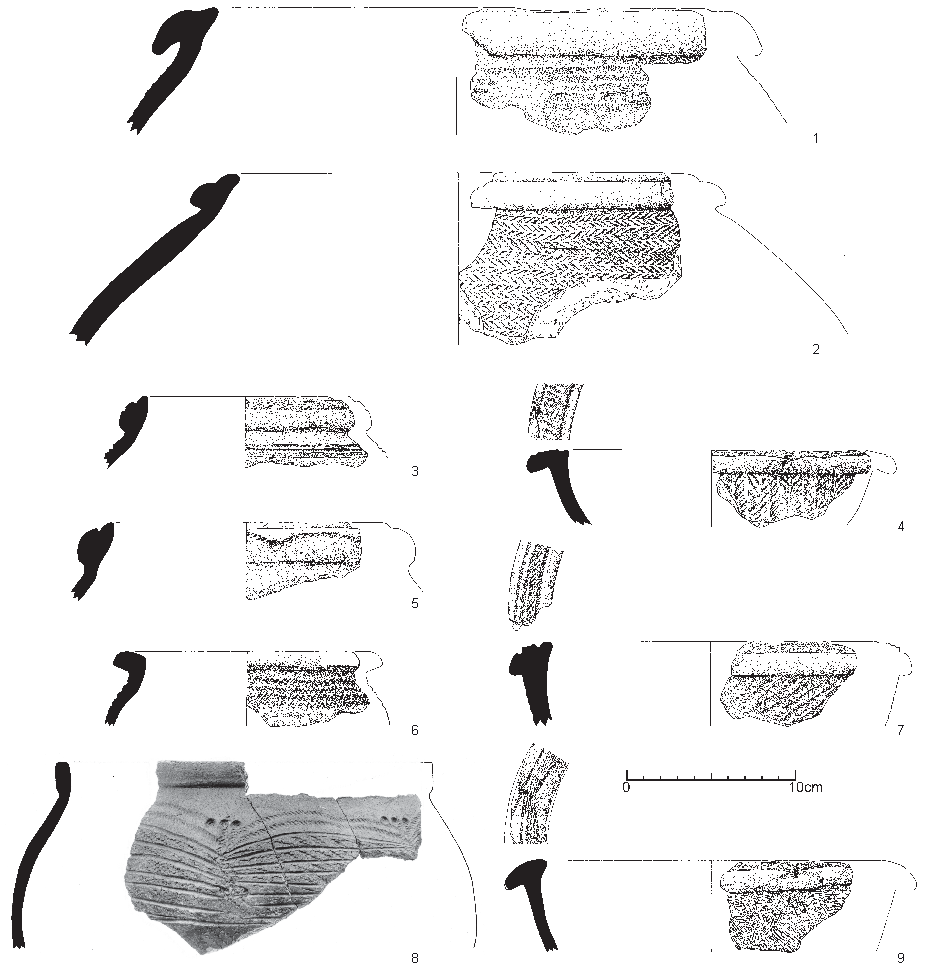
\includegraphics[width=\textwidth]{fig/MTB-Typen.pdf}
	\caption{Motenge-Boma-Gruppe: Vertreter aus Motenge-Boma.\\1:~Taf.~11.8; 2:~Taf.~11.7; 3:~Taf.~12.6; 4:~Taf.~14.5; 5:~Taf.~12.9; 6:~Taf.~12.4; 7:~Taf.~14.7; 8:~Taf.~16.2; 9:~Taf.~14.3.}
	\label{fig:MTB_Typvertreter}
\end{figure*}

\paragraph{Technologische Merkmale}\hspace{-.5em}|\hspace{.5em}%
Die GE der Motenge-Boma-Gruppe enthalten durchweg viel (39\,\%) bis sehr viel (57\,\%) nichtplastische Partikel, die fast ausschließlich den Größenklassen \textit{coarse} (63\,\%) und \textit{very coarse} (33\,\%) zuzurechnen sind. Bei den nichtplastischen Partikeln handelt es sich fast ausnahmslos um heterogene Sandmischungen auf Quarz-Basis (81\,\%). Nur in Einzelfällen finden sich auch Glimmer, Laterit oder ausgebrannte Organik in den Scherben. Die Keramik lässt sich vor allem den \textit{Fabrics} 5a (28\,\%), 4a (25\,\%) und 4c (18\,\%) zuordnen. Die Scherben der Motenge-Boma-Gruppe wurden zu großen Teilen aus rotbrennenden Tonen (34\,\%) gefertigt. Weißbrennende Tone sind deutlich seltener (18\,\%) beobachtet worden. Die übrigen Scherben zeigten häufig eine Mischung aus schwarzen, grauen, beigen und bräunlichen Farbtönen. Die Scherben zeigen grundsätzlich eine glatte (61\,\%) bis leicht raue (36\,\%) Oberfläche und die Wandungsdicke liegt im Mittel bei 8\,mm.


\paragraph{Formen}\hspace{-.5em}|\hspace{.5em}%
Das der Motenge-Boma-Gruppe zurechenbare Fundgut bestand zu großen Teilen aus Randscherben (71\,\%). Nur zwei GE konnten als hinreichend komplette Gefäße angesprochen werden. Insgesamt konnte bei 120~GE die Gefäßform bestimmt werden. Da das Material der \mbox{Motenge}-Boma-Gruppe aber zum großen Teil aus Randscherben bestand, war eine sichere Ansprache der Gefäßform nur in etwas über einem Drittel aller Fälle möglich (39\,\%). Etwa ein Fünftel aller Gefäße sind nicht näher bestimmbare flache Gefäße mit geschweifter Wandung (Typ~E; 21\,\%; Abb.~\ref{fig:MTB_Typvertreter}.6, 8; Taf.~12.2, 17.3, 19.1, 20.1--3). Unter den sicher bestimmten Gefäßformen fallen vor allem rundbodige, teilweise kleine Schälchen auf (Typ~I3--4; 38\,\%; Abb.~\ref{fig:MTB_Typvertreter}.4, 7, 9; Taf.~10.7, 15.5--7, 20.1--3). Mit Blick auf die Grundform machen diese Typen sowie andere schalenförmige Gefäße mit konvexer Wandung (Typ~I) 51\,\% des Inventars der Motenge-Boma-Gruppe aus. Schalenförmige Gefäße mit konvexer Wandung und einbiegendem Rand (Typ~H; Taf.~21.9--10) machen etwa 15\,\% aus, während Gefäße mit stark konvexer Wandung und ohne ausgeprägten Halsbereich (Typ~D; 8\,\%; Taf.~15.9, 19.3, 19.6), schalenförmige Gefäße mit abknickender Wandung (Typ~G; 3\,\%) und flaschenförmige Gefäße (Typ~A; 3\,\%; Taf.~17.6, 18.4) deutlich seltener vorkommen.

Der überwiegende Teil der Gefäße weist geschweifte bis konvexe Wandungen auf (74\,\%). Nur in Einzelfällen konnten andere Ausformungen des Bauchbereiches beobachtet werden. Die Randlippe ist häufig rund ausgeführt (M1; 40\,\%), während spitz zulaufende (M2; 23\,\%) und gerade abgestrichene Mündungen (M3; 22\,\%) seltener beobachtet wurden. Bei insgesamt 145~GE der Motenge-Boma-Gruppe wurde die Randform bestimmt. Grundsätzlich zeichnet sich die Motenge-Boma-Gruppe durch einen auffälligen Variantenreichtum in Bezug auf die Randgestaltung aus. Die bestimmende Randform sind stark umgelegte Ränder vom Typ B2.3 (29\,\%). Diese Randform findet sich fast ausschließlich an geschlossenen Gefäßen, die wiederum häufig keinen ausgeprägten Halsbereich aufweisen und dem Gefäßgrundtyp E zugerechnet werden können. Etwa 8\,\% aller GE zeigen stark umgeknickte, teilweise leicht nach unten gezogene Ränder vom Typ A2 (Abb.~\ref{fig:MTB_Typvertreter}.1,6; Taf.~11.10, 12.3, 19.3,6,8).\footnote{Eine gewisse Entsprechung für diese Randform lässt sich auch bei einer dem Botendo-Stil zugerechneten GE aus dem Befund NKI~2-1 in Nkile am Ruki (Fpl.~17) erkennen \parencite[150--158, 462 Taf.~28.3]{Wotzka.1995}.} Die Schalen vom Typ~I zeichnen sich häufig durch einbiegende Ränder mit einer heruntergezogenen Leiste an der Außenseite aus (A2.5). Diese Randgestaltung macht insgesamt 9\,\% aller beobachteten Formen aus. Etwas seltener konnten umgelegte oder verdickte Ränder (A2.4; 6\,\%) beobachtet werden. Des Weiteren fallen einbiegende Ränder auf, an deren Außenseite eine breite Wulst aufgelegt wurde (A4.4; Abb.~\ref{fig:MTB_Typvertreter}.3, 5; Taf.~12.7,11,13). Diese machen 5\,\% der beobachteten Ränder innerhalb der Motenge-Boma-Gruppe aus und wurden ausschließlich an Stücken dieser Stilgruppe beobachtet. Im gesamten Fundgut fanden sich lediglich zwei Bodenscherben, die sicher der Motenge-Boma-Gruppe zugewiesen werden konnten. In beiden Fällen handelt es sich um runde Böden vom Typ B1. Die bestimmenden Grundformen des Motenge-Boma-Stils sind große, rundbauchige Gefäße ohne Hals vom Typ E1 sowie kleine Schalen des Typs I3/I4.

\begin{figure*}[p]
	\centering
	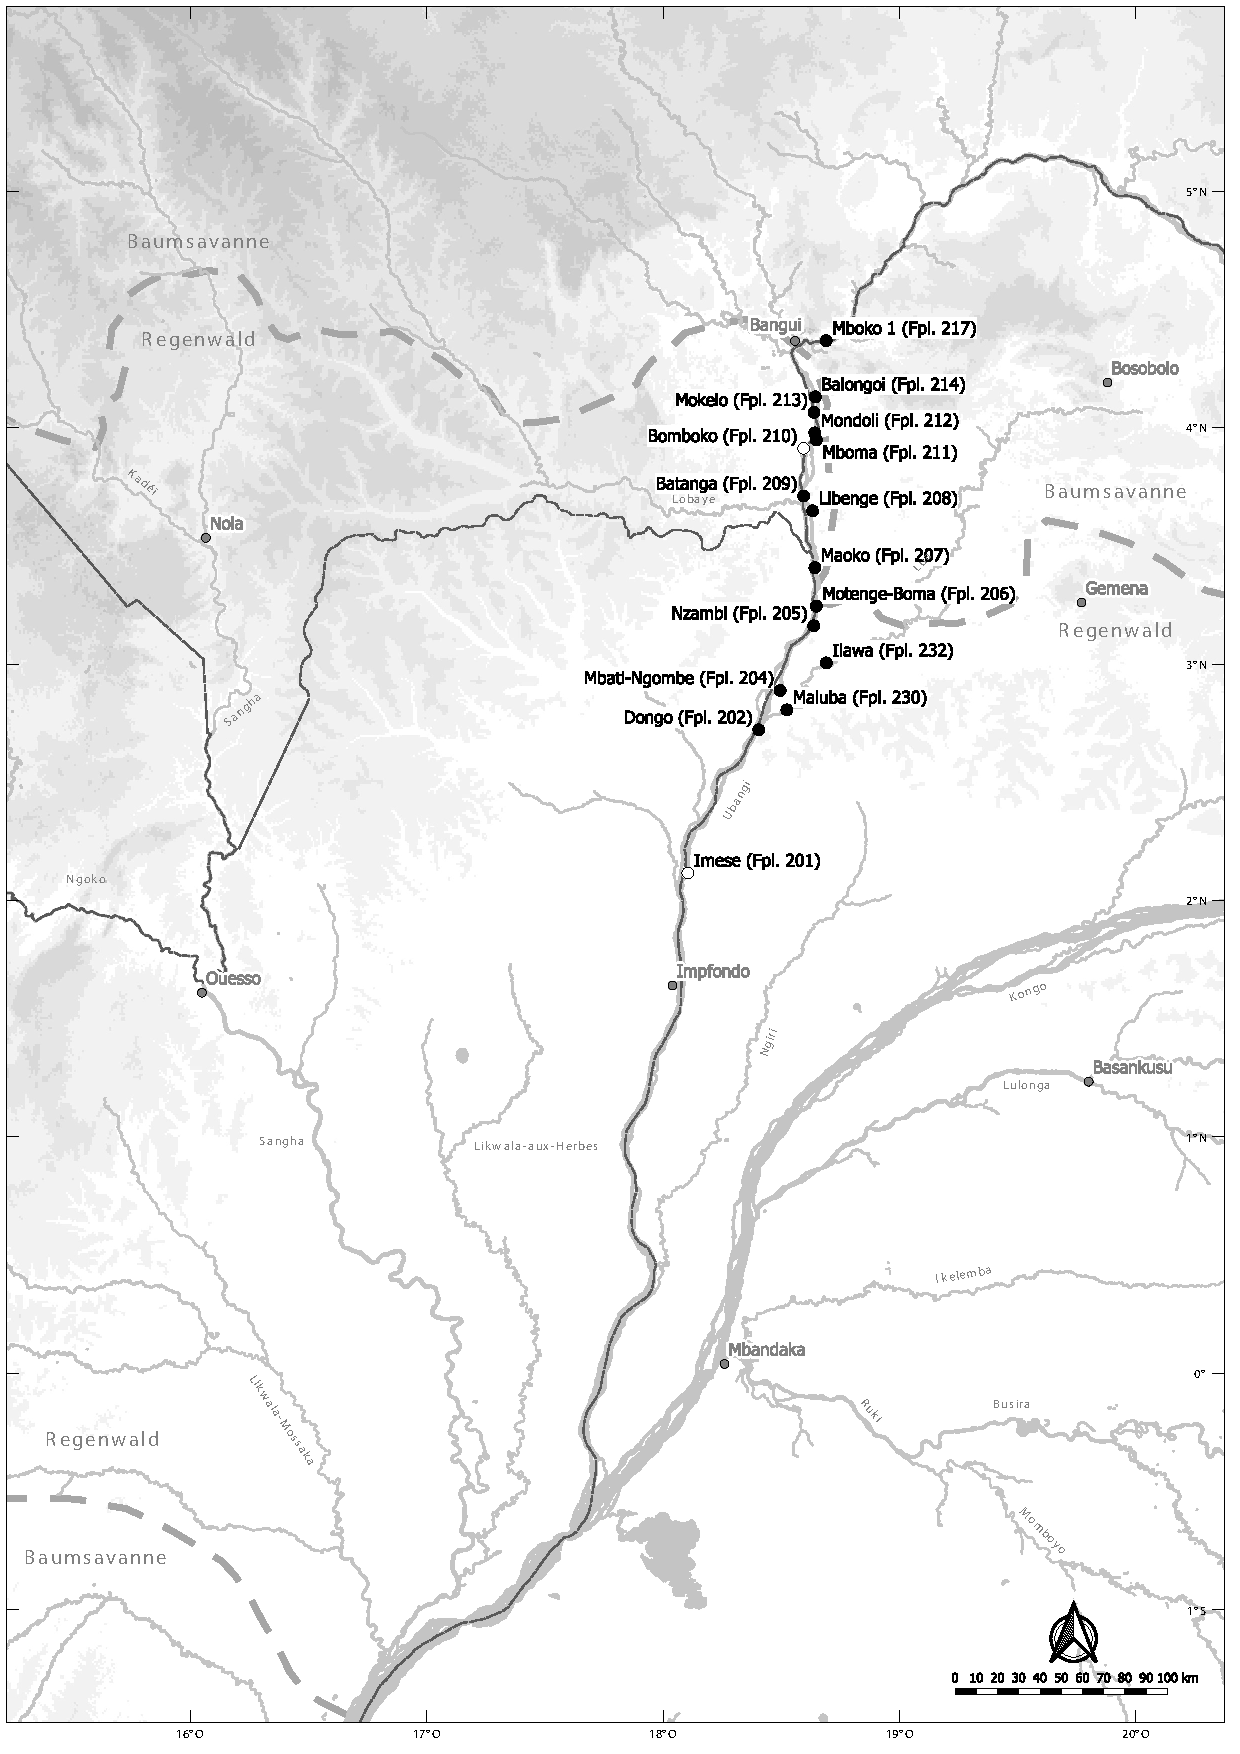
\includegraphics[width=\textwidth]{fig/MTB_Verbreitung.pdf}
	\caption{Motenge-Boma-Gruppe: Verbreitung.}
	\label{fig:MTB_Verbreitung}
\end{figure*}

\paragraph{Verzierungen}\hspace{-.5em}|\hspace{.5em}%
Eines der charakteristischen Merkmale der Motenge-Boma-Keramik ist das regelhafte Auftreten von Rouletteverzierungen, vor allem verschiedene Varianten von Schnitzroulette. Rouletteverzierungen machen zusammen mehr als 53\,\% aller beobachteten Verzierungselemente aus. Einzeln betrachtet bilden jedoch die fast ausschließlich an der Innenseite sowie außen im Randbereich angebrachten horizontalen Rillen das am häufigsten vertretene Verzierungselement (17\,\%; Tab.~\ref{tab:Verzierungselemente}: 02.1; Anlage~4\subref{fig:MTB_Verz}). Ebenfalls sehr häufig fanden sich Bögen eines rollrädchenartigen Motivs (Tab.~\ref{tab:Verzierungselemente}: 21.13; Abb.~\ref{fig:MTB_Typvertreter}.5), das 15\,\% aller Verzierungen ausmacht und ebenfalls größtenteils innen sowie außen an den Rändern zu beobachten ist. Diese beiden Verzierungselemente kommen regelhaft gemeinsam auf GE vor und heben sich von der vornehmlich auf den Schulter- und Bauchbereichen aufgetragenen Rouletteverzierung ab (Anlage~4\subref{fig:MTB_Verz}). Innerhalb der Roulettevierzierungen machen Varianten von Schnitzroulette (Tab.~\ref{tab:Verzierungselemente}: 21.5--13) mit fast 83\,\% aller Rouletteverzierungen den größten Anteil aus. Vegetabilisches \mbox{Roulette} findet sich deutlich seltener (Tab.~\ref{tab:Verzierungselemente}: 21.1--4; 16\,\%). Vornehmlich fand sich die Rouletteverzierung an den Schulter- und Bauchbereichen der Gefäße, in einigen Fällen aber auch auf der Innenseite der Ränder. Die häufigste Ausprägung von Rouletteverzierungen sind Schnitzroulette-Varianten, die ein tannenbaumartiges Muster \parencite[Tab.~\ref{tab:Verzierungselemente}: 21.12; 12\,\%; \textsc{Van Noten} 1982: Abb. 40.3; Abb.~\ref{fig:MTB_Typvertreter}.2, 4; siehe auch][Abb.~1.E]{LivingstoneSmith.2007} sowie eines mit gezähnten tiefen Einschnitten (Tab.~\ref{tab:Verzierungselemente}: 21.5--6; 12\,\%; Abb.~\ref{fig:MTB_Typvertreter}.1, 4, 6) erzeugen. Das häufigste vegetabilische \mbox{Roulette} ist \textit{knotted strip} (Tab.~\ref{tab:Verzierungselemente}: 21.1; 6\,\%; Abb.~\ref{fig:MTB_Typvertreter}.7; siehe auch ebd. 191 Abb.~1.C). Die übrigen Verzierungselemente kommen lediglich in sehr geringem Umfang vor. Charakteristisch für den Motenge-Boma-Stil ist eine Untergliederung der Gefäße durch spezifische Verzierungselemente. Während die Rouletteverzierungen auf die Schulter- und Bauchbereiche der Gefäße beschränkt sind, finden sich Rillen und Rollrädchen-Bögen vornehmlich innen und außen am Rand (Anlage~4\subref{fig:MTB_Verz}).


\paragraph{Datierung}\hspace{-.5em}|\hspace{.5em}%
Für die Keramik der Motenge-Boma-Gruppe liegen keine absoluten Datierungsansätze vor. Mit der Ausnahme von zwei GE stammen alle Funde aus Absammlungen rezenter Dorfflächen und lassen sich keinen Befunden zuweisen. Zwei Motenge-Boma-Scherben fanden sich in der teilweise untersuchten Grube MLB~85/103 (Kat.Nr.~5) in Maluba am Lua (Fpl.~230). Aus dem Befund wurden keine Proben zur Datierung und insgesamt auch nur 15 Scherben entnommen. Eine sichere Datierung der Motenge-Boma-Keramik ergibt sich aus diesem Befund demnach nicht, da in ihm älteres wie auch jüngeres Fundmaterial vermischt sind. Für \textcite[69]{vanNoten.1982d} weist die Keramik aus Motenge-Boma Parallelen zur rezenten Keramik der Region auf, ohne mit dieser aber vollends übereinzustimmen, was ihn zu einer subrezenten Datierung des Materials veranlasst. Im Rahmen dieser Arbeit ergaben sich keine entgegenlaufenden Indizien für die chronologische Ansprache des Motenge-Boma-Stils. Auffällig ist die teilweise ornamentale Überfrachtung von Gefäßen der Motengo-Boma-Gruppe. Sie unterscheiden sich darin deutlich von den eindeutig rezenten Stilen Dama und Mbati-Ngombe (Kap.~\ref{sec:DAM-Gr}--\ref{sec:MBN-Gr}). Ein Objekt aus der Sammlung zeitgenössischer Keramik des \textit{État Indépendant du Congo}, die sich im Besitz des damaligen \textit{Musée du Congo} befindet, zeigt die für die Motenge-Boma-Keramik charakteristische rollrädchenartige Verzierung, unterscheidet sich jedoch in allen anderen Charakteristika \parencite[Taf.~XIV.204]{Coart.1907}. Es kann daher lediglich nur von einer sehr isolierten Weitergabe der Eigenschaften des Motenge-Boma-Stils in die zeitgenössische Keramik ausgegangen werden. In der Zusammenschau der vorliegenden Indizien kann für die Motenge-Boma-Keramik lediglich eine provisorische, das 15. bis 18. Jh. n.~Chr. abdeckende Datierung vorgeschlagen werden.


\paragraph{Verbreitung}\hspace{-.5em}|\hspace{.5em}%
Die Motenge-Boma Gruppe weist ein stark begrenztes Verbreitungsgebiet entlang des oberen \mbox{Ubangi} auf (Abb.~\ref{fig:MTB_Verbreitung}). Das südliche Ende ihrer Verbreitung findet sich in \mbox{Dongo} (Fpl.~202) im Bereich der Lua-Mündung, während es in Richtung Norden bis Mboko~I (Fpl.~217) bei Bangui reicht. Über dieses Kerngebiet heraus sind, bis auf einen fragliche GE in Imese (Fpl.~201), keine weitere Funde der Motenge-Boma-Gruppe bekannt.
